\documentclass[preprint,12pt]{elsarticle}

\usepackage[T1]{fontenc}
\usepackage{lmodern}
\usepackage{amsmath,amssymb}
\usepackage{booktabs}
\usepackage{graphicx}
\usepackage{microtype}
\usepackage{tabularx}
\usepackage{array}
\usepackage{xcolor}
\usepackage{hyperref}
\usepackage{placeins}
\setlength{\emergencystretch}{3em}

\journal{Advanced Engineering Informatics}
\graphicspath{{figures/}}
\newcolumntype{Y}{>{\raggedright\arraybackslash}X}
\newcommand{\cai}{\mathrm{CAI}}
\newcommand{\auebc}{\mathrm{AUEBC}}
\newcommand{\risk}{\mathcal{R}}
\newcommand{\legal}{\mathcal{I}}
\newcommand{\actions}{\mathcal{A}}

\begin{document}

% Front matter and Section 1 are drafted after the numerical results freeze.
\section{Introduction}
\label{sec:introduction}

\section{Related Research and Problem Formulation}
\label{sec:related-formulation}

\subsection{Ultrasonic information for post-impact performance assessment}
\label{sec:related-cai}

Low-velocity impact can leave limited visible evidence while producing a
spatially distributed internal damage state that affects compression-after-
impact (CAI) performance. Surface profiles have consequently been studied as
accessible predictors of internal impact damage and residual CAI strength
\cite{hasebe2022internal,hasebe2025compression}. These mappings establish that
surface observations can be useful within a defined cohort, but they do not
make the surface and internal fields informationally equivalent. Image-resolved
analyses of impacted laminates likewise motivate retaining spatial morphology
rather than reducing damage to a single projected extent
\cite{bull2018image}.

The paired public releases used here provide specimen metadata, surface
profiles, ultrasonic C-scans, and CAI measurements
\cite{hasebe2022dataset,hasebe2025caidataset}. Mack et al. subsequently showed
that full C-scan images can support direct prediction of impact energy and CAI
strength with a convolutional model \cite{mack2026cscan}. That study is the
closest application-level precedent: it establishes full-image predictive
feasibility, so the present contribution is not the use of C-scans or image
features for CAI regression. The unresolved engineering-information question
is narrower and different. It asks which portions of the measured field carry
task value, whether the value of an unacquired portion can be inferred from a
legal partial inspection state, and whether that estimate improves the next
measurement decision across held-out experimental domains.

This distinction also separates a predictive input from an acquisition
policy. A full-field model may quantify the information available after the
inspection has ended, but it does not tell an inspector which location to
measure next or whether the value assigned to that location can be known before
measurement. Those propositions require different information sets and
different controls.

\subsection{Sparse and adaptive ultrasonic inspection}
\label{sec:related-adaptive}

Sparse ultrasonic sampling has been used to recover impact-delamination
patterns from incomplete measurements \cite{nguyen2025sparse}. Recent adaptive
sampling of composite Lamb wavefields combines a damage-guided sampling pattern
with a spatial--temporal masked autoencoder, with full-wavefield reconstruction
as the learning endpoint \cite{ji2026adaptive}. Autonomous robotic ultrasonic
inspection has also selected successive physical locations using Bayesian
optimization over a damage-probability or novelty field
\cite{fuentes2020autonomous}. Adaptive and sequential ultrasonic inspection are
therefore established; neither is a priority claim of this work.

The acquisition objective matters. Reconstruction-oriented sampling rewards a
measurement when it improves the recovered signal or image. Damage-localization
sampling rewards evidence that resolves the presence or position of a defect.
The present CAI task instead rewards measurements that reduce residual-capacity
prediction error. These objectives can select the same locations, but this
agreement cannot be assumed. A visually or numerically accurate reconstruction
may preserve features irrelevant to CAI, whereas a mechanically useful
measurement need not minimize global image error. We therefore compare
mechanics- and reconstruction-conditioned utilities under a common acquisition
and cost contract.

Sparse fractions in this paper refer to locations on a registered digital
raster. They are not converted into scanner time. Physical travel, coupling,
settling, pulse repetition, and path-planning overhead are absent from the
released data, so a native-raster measurement reduction is not evidence of an
equal inspection-time reduction.

\subsection{Task-driven sensing and value of information}
\label{sec:related-voi}

Task-driven experimental design explicitly chooses measurements for a
downstream objective rather than for signal reconstruction alone. For example,
TADRED selects a compact global channel design from dense multi-channel images
while optimizing a user-specified task \cite{blumberg2024experimental}. In
ultrasonic structural health monitoring, value-of-information criteria have
been used to trade diagnostic information against the number and placement
cost of guided-wave sensors \cite{cantero2020optimal}. These works establish
both task-driven imaging and ultrasonic value-of-information design as prior
art.

Sequential decision making adds a further dependency: the value of a future
observation depends on what is already known. In a partially observable
infrastructure-management setting, component inspection, monitoring, and
system-level scheduling are distinct decisions because beliefs and future
opportunities evolve after observations \cite{memarzadeh2016value}. This
separation is directly relevant to partial C-scan inspection. A retrospective
calculation may show that a location would have reduced CAI error, while a
deployable score may fail to identify that location from the current state;
even an accurate one-step score may fail when measurements must be selected as
a cost-constrained set.

Accordingly, this paper does not present task-driven acquisition itself as the
novelty. Its contribution is an evidence hierarchy that separates three claims
often collapsed in engineering machine learning: whether information is useful
to a task, whether its conditional value is observable before acquisition, and
whether the resulting estimate is actionable in a bounded sensing decision.

\subsection{Problem formulation and research questions}
\label{sec:problem-formulation}

Let specimen $i$ belong to experimental domain $d(i)$. Its response $y_i$ is
the damaged-to-intact CAI-strength ratio. Let $z_i$ denote legal pre-inspection
context, $S_i$ the complete native-raster ultrasonic field, and
$\legal_{i,t}$ the information legally available after acquisition step $t$.
The latter contains $z_i$, acquired coordinates and values, action history, and
exact cost, but excludes unrevealed values in $S_i$ and the outcome $y_i$. A
candidate measurement $X\in\actions(\legal_{i,t})$ is legal only if it refines
the current hierarchical measurement state without exceeding the budget.

For a fixed downstream predictor $f$ and task loss $\ell$, define the risk of a
state as
\begin{equation}
  \risk_f(\legal_{i,t}) = \ell\!\left(y_i,
  f(\legal_{i,t})\right).
  \label{eq:state-risk}
\end{equation}
The realized task value of candidate $X$ is
\begin{equation}
  U_f(X\mid\legal_{i,t}) =
  \risk_f(\legal_{i,t})-
  \risk_f(\legal_{i,t}\cup X).
  \label{eq:task-value}
\end{equation}
A positive value means that revealing $X$ reduces error for this predictor at
this state. Because both terms depend on $f$, Eq.~\eqref{eq:task-value} defines
\emph{downstream-predictor-conditioned task value}; it is not an intrinsic or
universal mechanical property of a location. During retrospective analysis,
$U_f$ may use the true response and counterfactual revealed measurements. Such
values are teacher or oracle evidence and are unavailable to a deployable
policy.

The study addresses three research questions:
\begin{description}
  \item[RQ1 --- Useful:] What ultrasonic information is useful for CAI
  assessment, and does the optimal acquisition objective depend on the
  downstream task?
  \item[RQ2 --- Observable:] Can the value of a future measurement be inferred
  from the information legally available at the current inspection state?
  \item[RQ3 --- Actionable:] Can conditionally valued information be converted
  into a better cost-constrained sensing decision?
\end{description}
These questions are ordered but not logically equivalent. Evidence for RQ1
provides a target for RQ2; it does not guarantee that the target can be
estimated. Evidence for RQ2 provides a score for RQ3; it does not guarantee
that greedy, planned, or feedback-driven selections improve the final
cost--error trajectory.

\section{Task-Relevant Information Hierarchy and Operational Framework}
\label{sec:framework}

\subsection{Framework overview}
\label{sec:hierarchy-overview}

The Task-Relevant Information Hierarchy in Fig.~\ref{fig:hierarchy} treats
Useful, Observable, and Actionable as separate empirical layers. At the first
layer, a measurement is useful if access to it improves a defined engineering
task under a fixed predictor and validation protocol. At the second, its
conditional value is observable if a score computed only from legal current
information agrees with a strict out-of-fold retrospective target. At the
third, the score is actionable if using it in a cost-constrained policy improves
the complete decision trajectory relative to deployable controls.

\begin{figure}[t]
  \centering
  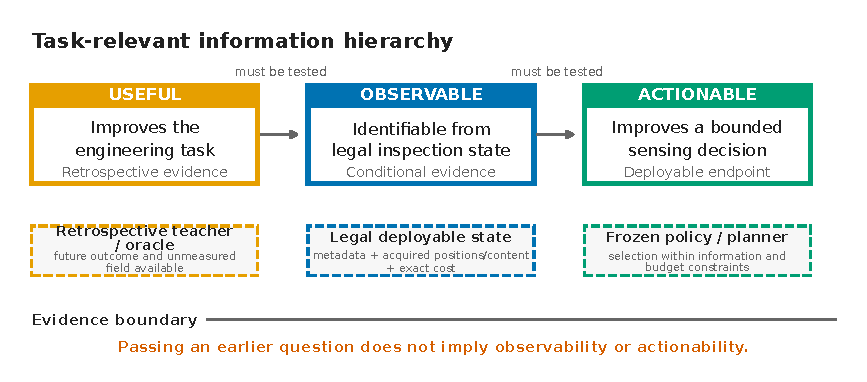
\includegraphics[width=\textwidth]{figure1_information_hierarchy.pdf}
  \caption{Task-relevant information hierarchy. Useful information improves the
  engineering task, observable information can be inferred from legally
  available inspection state, and actionable information improves a bounded
  sensing decision. Retrospective teacher/oracle evidence is separated from the
  deployable state and policy; passing one question does not imply the next.}
  \label{fig:hierarchy}
\end{figure}

The hierarchy is deliberately fail-closed. A result at one layer authorizes a
question at the next layer, not a success claim. This prevents a retrospective
oracle from being presented as a policy, a high rank correlation from being
presented as improved acquisition, or lower reconstruction error from being
presented as higher structural-performance value.

\subsection{Downstream-predictor-conditioned task usefulness}
\label{sec:framework-useful}

Usefulness is assessed by changing the information available to the downstream
task while holding the cohort, held-out domains, response, and validation
logic fixed. The first comparison asks whether a spatial internal field adds
CAI-relevant information beyond a matched scalar representation. The second
asks how much of the registered full-field gain remains under a fixed sparse
sampling and interpolation protocol. These are predictive information
comparisons; neither identifies a deployable adaptive acquisition rule.

For candidate designs, the corresponding retrospective oracle chooses
\begin{equation}
  X^*_{f,i,t} = \arg\max_{X\in\actions(\legal_{i,t})}
  U_f(X\mid\legal_{i,t})
  \quad \text{subject to}\quad c(X\mid\legal_{i,t})\leq b_t,
  \label{eq:oracle-action}
\end{equation}
where $c$ is exact added native-raster cost and $b_t$ is the remaining budget.
Because evaluation of Eq.~\eqref{eq:oracle-action} requires counterfactual
measurements and $y_i$, it measures headroom rather than deployability.
Applying the same acquisition contract to CAI error and image-reconstruction
error tests whether utility is task-specific. Repeating the value calculation
with different downstream predictors tests whether the map is stable to the
definition of $f$.

\subsection{Conditional observability}
\label{sec:framework-observable}

Observability concerns an estimate, not the retrospective value itself. Let
$g_\theta$ be a scorer with inputs restricted to the legal state and a candidate
descriptor. Its prediction is
\begin{equation}
  \widehat U_{i,t,X}=g_\theta\!\left(
  \legal_{i,t},X,c(X\mid\legal_{i,t})\right).
  \label{eq:value-scorer}
\end{equation}
Training labels are generated strictly out of fold: for each outer target
domain, teacher predictors and scorer selection use source domains only. The
held-out domain is queried after all fitting and selection are fixed. Agreement
with the teacher is examined through within-specimen candidate ranking,
best-action and top-$k$ agreement, and exact-budget set regret.

Conditional observability has two potential failure modes. First, a static
pre-acquisition representation may contain insufficient specimen-specific
information to rank future measurements. Second, the target itself may evolve
as observations accumulate. We therefore measure teacher-value turnover across
states before asking whether a dynamic scorer tracks it. Matched positions-only,
reconstruction, static, and shuffled-content controls distinguish access to
acquisition geometry from evidence attributable to newly measured specimen
content. These controls bound the claim: improvement relative to an empty state
does not establish content-specific observability if geometry or shuffled
content performs as well or better.

\subsection{Decision actionability}
\label{sec:framework-actionable}

Actionability evaluates the policy produced by a score. At state
$\legal_{i,t}$, a deployable selector chooses a legal candidate using current
information and exact incremental cost. A one-step value-per-cost rule is
\begin{equation}
  \pi(\legal_{i,t}) = \arg\max_{X\in\actions(\legal_{i,t})}
  \frac{\widehat U_{i,t,X}}{c(X\mid\legal_{i,t})}.
  \label{eq:policy}
\end{equation}
The registered testbed also evaluates direct cost-aware scores and bounded
lookahead, but all choices obey the same reveal and budget contract.

Policy quality is measured over the complete error--budget curve rather than at
one convenient endpoint. For checkpoints $q_1<\cdots<q_K$ with CAI errors
$e_i(q_k)$, the per-specimen area under the error--budget curve is computed by
trapezoidal integration,
\begin{equation}
  \auebc_i = \sum_{k=1}^{K-1}
  \frac{e_i(q_k)+e_i(q_{k+1})}{2}\,(q_{k+1}-q_k),
  \label{eq:auebc}
\end{equation}
with lower values preferred. Component substitutions compare learned and
retrospective valuation or planning under a bounded diagnostic. They locate
decision headroom but remain non-deployable when true future values enter.
Feedback is tested separately because re-scoring after each reveal can help
only if the state update carries usable specimen-specific information and the
scorer responds to it appropriately.

\subsection{Operationalization with causal partial-state measurement valuation}
\label{sec:framework-operationalization}

MAVIS is used here as a frozen operational testbed for state-conditioned
valuation and actionability, not as a demonstrated superior adaptive scanner.
Its authority layer issues two non-overlapping views. The deployable policy
context contains specimen metadata and surface/context features but contains no
complete scan or CAI outcome. A separate source-teacher view exposes the full
scan and outcome only to source-domain teacher construction and retrospective
evaluation. The held-out evaluation view is not accepted by policy or state
encoder interfaces.

Causal reveal begins with a geometry-neutral uniform scout. The native raster
is partitioned into 64 cells; each cell has a three-level refinement state.
Only coordinates implied by the initial scout and subsequent legal actions are
materialized. Revealed coordinates and RGB values, measurement levels, action
history, native shape, and exact acquired count form an immutable inspection
state. A state bank records these histories at the registered checkpoints.

The current-state encoder aggregates variable-length measured tokens with a
permutation-invariant DeepSets model and fuses them with context and exact-cost
features. The mechanics head predicts CAI from the same causally available
state. For source domains, a strict-OOF teacher evaluates each legal candidate
using
\begin{equation}
  u_{i,t,X} =
  \left|y_i-\widehat y_i(\legal_{i,t})\right|-
  \left|y_i-\widehat y_i(\legal_{i,t}\cup X)\right|.
  \label{eq:teacher-value}
\end{equation}
The dynamic scorer receives the encoded current state and candidate geometry,
level transition, exact added cost, and remaining cost. It predicts both a raw
selection score and the teacher value. Rollout applies the selected legal
action, reveals only its registered coordinates, updates the state, and either
re-scores with feedback or retains the frozen initial ordering for the
no-feedback control.

This implementation makes the information boundary executable. Future scan
content and the true CAI outcome are necessary for teacher labels and oracle
diagnostics, but they cannot enter the deployable scorer or rollout. The
observability and actionability claims are consequently evaluated against the
same causal state that would be available at the corresponding digital
inspection step.

\section{Multi-Domain CFRP Case Study and Experimental Design}
\label{sec:case-study}

\subsection{Specimens and ultrasonic/CAI measurements}
\label{sec:specimens}

The case study uses 276 CAI-complete carbon-fiber-reinforced polymer specimens
from six released experimental datasets
\cite{hasebe2022dataset,hasebe2025caidataset}. The domains contain 45, 49, 43,
59, 42, and 38 specimens, respectively. They differ in laminate configuration
and experimental conditions and are retained as indivisible validation units.
The response is the damaged-to-intact CAI-strength ratio. Available modalities
are specimen metadata, surface observables, an ultrasonic RGB C-scan of the
internal damage field, and the CAI outcome.

The registered scan manifest binds every specimen identifier to its domain,
native raster shape, pixel count, and source-content hashes. Native rasters are
not resized for acquisition-cost accounting. This matters because scan sizes
vary across the cohort: a nominal percentage alone does not specify the number
of newly observed locations. Table~\ref{tab:case-protocol} summarizes the
cohort and evaluation contract.

\begin{table*}[t]
\centering
\caption{Case study and evaluation protocol.}
\label{tab:case-protocol}
\small
\setlength{\tabcolsep}{4pt}
\begin{tabularx}{\textwidth}{@{}>{\RaggedRight\arraybackslash}p{0.20\textwidth}X@{}}
\toprule
Item & Value \\
\midrule
Cohort & 276 physical specimens across 6 experimental domains; domain counts 45, 49, 43, 59, 42, 38 \\
Information representations & Specimen metadata and surface observables; full ultrasonic C-scan field; 25\% normalized-raster sparse field; current partial state \\
Actions and cost & 8 x 8 cells with three acquisition levels; cost is exact unique native-raster locations divided by native count, with no scanner-time equivalence \\
Information boundary & Deployable state contains metadata, acquired positions and content, legal actions, and exact cost; teacher and oracle information is retrospective and non-deployable \\
Evaluation & Strict nested leave-one-domain-out (LODO); outer-domain outcomes are excluded from training, selection, and calibration \\
Statistics & physical specimen first and held-out domain second; equal-domain aggregation with synchronized within-domain bootstrap; repeated computational records are not independent samples \\
\bottomrule
\end{tabularx}
\end{table*}


\subsection{Information representations and candidate measurements}
\label{sec:representations}

The usefulness experiments compare three information resolutions. The scalar
reference combines metadata, surface observations, and scalar summaries of the
internal scan. The matched spatial candidate uses the same registered predictor
family but retains the selected full C-scan field representation. A separate
internal-only field estimator is reported only as a sensitivity path; it is not
substituted for the matched confirmatory comparison. The sparse retrospective
condition reveals a registered 25% sampling pattern on a normalized raster and
uses bilinear interpolation before applying the frozen field pathway.

For sequential acquisition, each native raster is divided into an $8\times8$
cell grid. A cell may move through three registered sampling levels, and an
action refines exactly one cell by one level. Candidate descriptors contain the
cell position, level transition, exact number of newly observed native
locations, native count, and remaining exact budget. This representation
permits comparison of uniform, random, reconstruction-conditioned,
mechanics-conditioned, static, and state-conditioned choices without changing
the legal action space.

Mechanics utility is the change in CAI prediction loss in
Eq.~\eqref{eq:task-value}. Reconstruction utility uses normalized RGB mean
squared error over the same registered raster. These utilities are kept
separate: an acquisition may be optimal for one and suboptimal for the other.

\subsection{Whole-dataset generalization protocol}
\label{sec:lodo}

All headline results use leave-one-domain-out (LODO) evaluation. Each of the six
experimental datasets serves once as the outer target domain. Model fitting,
normalization, hyperparameter or checkpoint selection, teacher construction,
policy choice, and fallback thresholds use only the other five source domains.
The outer-domain outcomes are excluded until the frozen candidate is evaluated.
When an inner selection loop is required, entire source domains remain intact.
This nested structure avoids the optimistic error estimates that arise when
model selection and assessment reuse observations \cite{varma2006bias} and
aligns the validation unit with the intended unseen-experiment question rather
than a specimen-random split \cite{gulrajani2021domainbed}.

The physical specimen is the primary statistical unit. Multiple candidate
actions, random seeds, and checkpoints for one specimen are repeated
computational records, not independent samples. Domain effects are first
computed from paired specimen outcomes inside each held-out domain and then
aggregated with equal weight across the six domains.

\subsection{Privileged, deployable, and forbidden information}
\label{sec:information-boundary}

The information boundary is defined by when and where a variable is available.
Metadata and surface observables are legal before ultrasonic acquisition.
Acquired positions, measured RGB values, measurement levels, legal actions, and
exact current cost are deployable state variables. Reconstructions from that
legal state may be used as controls. Unacquired ultrasonic content and the true
CAI outcome are forbidden to a deployable scorer or policy.

Teacher and oracle analyses deliberately use privileged information to define
retrospective targets and headroom. Their outputs are never described as
deployable. In particular, a true-value oracle may inspect counterfactual
outcomes for all legal actions, and a joint near-oracle may compare reachable
action sets. These rows answer whether an opportunity exists or where a bounded
decision gap lies; they do not specify an implementable inspector.

\subsection{Exact acquisition cost, metrics, and statistical inference}
\label{sec:metrics}

The registered checkpoints are 3.125%, 6.25%, 9.375%, 12.5%, 18.75%, and 25%
of the native raster. Initial scouts are 1.5625% except in the one domain whose
native geometry requires a 3.125% scout. At every transition, cost is the number
of unique newly revealed native-raster coordinates. Effective budget is that
count divided by the specimen's native pixel count. Previously observed
coordinates have zero added cost, and an action that would exceed the current
cap is illegal. No result is translated into physical scanner time.

For full-field and sparse prediction, the primary outcome is equal-domain mean
absolute error in CAI ratio. Sequential CAI performance is summarized by
$\auebc$ from Eq.~\eqref{eq:auebc}; lower values are better. Reconstruction is
measured by normalized RGB mean squared error. Observability metrics include
Spearman rank agreement between predicted and strict-OOF teacher action values,
best-action turnover or agreement, top-$k$ overlap, and exact-budget set regret.
Actionability contrasts use paired differences in specimen $\auebc$.

Uncertainty intervals use synchronized bootstrap resampling of physical
specimens within each held-out domain. The same resampled indices are applied
to both methods in a contrast, domain means are recomputed, and the six domain
means are equally weighted. The registered scalar-to-field family uses its
predeclared familywise simultaneous interval. Other intervals retain the
registered paired-bootstrap definitions. With only six domains, domain counts
are always reported beside the aggregate effect rather than treated as a
large-sample inferential substitute; this is consistent with the caution
required for clustered data with few groups \cite{huang2018cluster}.

\subsection{Validation matrix for RQ1--RQ3}
\label{sec:validation-matrix}

RQ1 combines the matched scalar-to-spatial contrast, sparse-retention boundary,
retrospective acquisition headroom, cross-objective oracle specificity, and
downstream-predictor sensitivity. RQ2 combines static value observability,
teacher-value evolution, matched positions/reconstruction controls, and
dynamic/static/shuffled scoring controls. RQ3 combines retrospective component
substitution, bounded set planning, feedback, and the frozen policy comparison
against the strongest deployable baseline.

This matrix prevents evidence migration between layers. Oracle headroom cannot
support a deployable policy claim; a dynamic score cannot support
content-specific observability if its matched adverse controls remain stronger;
and a planning diagnostic cannot support improved acquisition unless the
frozen end-to-end policy also improves. Section~\ref{sec:results-discussion}
reports the three answers in this order.

% Section 5 is drafted only from the canonical metric authority.
\section{Experimental Results and Discussion}
\label{sec:results-discussion}

% Section 6, the abstract, and the final title are drafted after Section 5.
\section{Conclusions}
\label{sec:conclusions}

\bibliographystyle{elsarticle-num}
\bibliography{references}

\end{document}
